%\chapter{Macrofísica: Objetos Compactos}
%\thispagestyle{fancy}

% Marco teórico - Macrofísica


%\section{Relatividad General}


%\section{Solución de Schwarzschild}


%\section{Ecuaciones de Estructura}

%\section{Observaciones de Estrellas de Neutrones}

%masas, radios, etc.

\chapter{Macrofísica: Objetos Compactos}

Los objetos compactos representan uno de los laboratorios naturales más extremos del universo, en los que la materia alcanza densidades, presiones y energías extremas que permiten extender nuestra comprensión de la física fundamental. Las estrellas de neutrones, en particular, constituyen el resultado final del colapso gravitacional de estrellas masivas, comprimiendo la materia a densidades que alcanzan varios órdenes de magnitud por encima de la densidad nuclear, en entornos de presión y temperatura que son extremadamente difíciles de reproducir en laboratorios terrestres \cite{baadeSuperNovae1934}. El estudio de estos objetos requiere necesariamente del escenario de la Relatividad General de Einstein, donde la curvatura del espacio-tiempo responde al contenido energético del sistema y viceversa.

En este capítulo desarrollamos los fundamentos teóricos necesarios para describir la estructura y propiedades de las estrellas de neutrones desde una perspectiva macroscópica. Comenzamos con una revisión de los fundamentos de la Relatividad General, estableciendo las ecuaciones de campo de Einstein que gobiernan la dinámica del espacio-tiempo. Posteriormente, exploramos la forma general de geometrías esféricamente simétricas, que proporciona un modelo básico para comprender la estructura de los objetos compactos. A partir de estos fundamentos, derivamos las ecuaciones de estructura que relacionan las propiedades microscópicas de la materia con las características macroscópicas observables de las estrellas de neutrones. Todas las secciones anteriores están fundamentadas en base al texto de Misner et al. \cite{misnerGravitation2017}. Finalmente, presentamos una revisión de las observaciones astronómicas más relevantes que han refinado nuestro entendimiento de estos objetos en la última década.

\section{Relatividad General}

La teoría de la Relatividad General, formulada por Einstein en 1915 \cite{einsteinFeldgleichungenGravitation1915}, es la descripción más exitosa de la gravitación como manifestación de la curvatura del espacio-tiempo. Esta teoría establece que la presencia de materia y energía modifica la geometría del espacio-tiempo, y que esta curvatura, a su vez, determina el movimiento de la materia y la propagación de la energía. La Relatividad General se fundamenta en dos principios básicos: el principio de equivalencia, según el cual los efectos de un campo gravitacional uniforme son localmente indistinguibles de los efectos de una aceleración uniforme, permitiendo que la gravitación pueda ser ``eliminada'' localmente mediante la elección apropiada de un sistema de coordenadas en caída libre; y el principio de covariancia general, el cual exige que las leyes de la física tengan la misma forma en todos los sistemas de coordenadas, requiriendo que las ecuaciones de la teoría sean expresadas en términos de tensores para asegurar su invariancia bajo transformaciones generales de coordenadas. Una representación esquemática del principio de equivalencia puede verse en la figura \ref{fig:equivalence_principle}, donde la esfera roja aparentemente cae en ambos sistemas, uno es un cohete acelerado, el otro la superficie de la tierra, siendo los dos sistemas de referencia indistinguibles.

\begin{figure}[h]
	\centering
	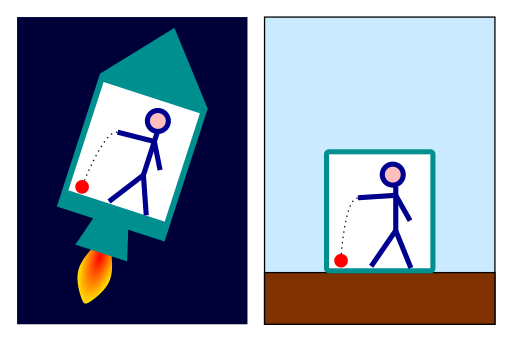
\includegraphics[width=0.7\linewidth]{Figuras/512px-Elevator_gravity.svg}
	\caption{Representación esquemática del principio de equivalencia. Markus Poessel.}
	\label{fig:equivalence_principle}
\end{figure}

\subsection{Ecuaciones de Campo de Einstein}

Las ecuaciones de campo de Einstein son un conjunto de ecuaciones diferenciales no lineales cuya forma compacta es:

\begin{equation}
	G_{\mu\nu} = 8\pi T_{\mu\nu},
	\label{eq:einstein_field}
\end{equation}

donde $G_{\mu\nu} = R_{\mu\nu} - \frac{1}{2}Rg_{\mu\nu}$ es el tensor de Einstein construido a partir del tensor de Ricci $R_{\mu\nu}$ y el escalar de curvatura $R$, y $T_{\mu\nu}$ es el tensor de energía-momento que describe las propiedades de la materia y energía presentes en el espacio-tiempo. Este conjunto de ecuaciones describe cómo la distribución de materia y energía determina la curvatura del espacio-tiempo, y cómo esta curvatura afecta el movimiento de la materia y la energía de vuelta. Las ecuaciones de Einstein satisfacen automáticamente las leyes de conservación del momentum y la energía a través de la identidad de Bianchi $G_{\mu\nu}{}^{;\rho} = 0$, lo que implica:

\begin{equation}
	\nabla_\rho T^{\mu\nu} = T^{\mu\nu}{}_{;\rho} = 0.
\end{equation}

Para describir la materia en el interior de las estrellas de neutrones, consideramos un modelo de fluido perfecto. El tensor de energía-momento es:

\begin{equation}
	T_{\mu\nu} = (\rho + P)u_\mu u_\nu - Pg_{\mu\nu},
	\label{eq:tensor_fluido_perfecto}
\end{equation}

donde $\rho$ es la densidad de energía del fluido, $P$ es la presión isótropa, y $u^\mu$ es la cuadrivelocidad del fluido, normalizada según $u^\mu u_\mu = 1$. Esta descripción asume que no hay flujos de calor, viscosidad, ni esfuerzos de corte en el fluido, aproximación válida para escalas de tiempo mucho mayores que los tiempos de relajación hidrodinámicos.

\section{Simetría Esférica}

Para describir la estructura de las estrellas de neutrones, vamos a resolver las ecuaciones de Einstein asumiendo simetría esférica y condiciones estáticas. La forma general de estas soluciones establece el punto de partida para entender tanto el interior como el exterior de objetos compactos con simetría esférica, en el marco de la teoría de la relatividad general. El elemento de línea de un sistema estático y esféricamente simétrico puede escribirse como:

\begin{equation}
	ds^2 = e^{2\phi(r)}dt^2 - e^{2\lambda(r)}dr^2 - r^2(d\theta^2 + \sin^2\theta d\varphi^2),
	\label{eq:metrica_esferica_general}
\end{equation}

donde $\phi(r)$ y $\lambda(r)$ son funciones arbitrarias de la coordenada radial $r$, y hemos utilizado coordenadas esféricas $(t,r,\theta,\varphi)$. La simetría esférica impone que la métrica sea invariante bajo rotaciones en el grupo $SO(3)$, mientras que la condición estática requiere la ausencia de términos cruzados $dt dr$, $dt d\theta$, y $dt d\varphi$, así como independencia explícita de la coordenada temporal. La métrica (\ref{eq:metrica_esferica_general}) representa la forma más general compatible con estas simetrías \cite{misnerGravitation2017}. Una representación gráfica de la geometría del espacio-tiempo que contiene una estrella con simetría esférica, estática, puede apreciarse en la figura \ref{fig:geometry-misner}, donde la región blanca representa la geometría exterior (fuera de la estrella), y la zona gris la región interior (dentro de la estrella).


%Para la métrica esféricamente simétrica (\ref{eq:metrica_esferica_general}), las componentes no triviales del tensor de Ricci son:
%
%\begin{align}
%	R_{tt} &= e^{2(\phi-\lambda)}\left[\phi'' + \phi'^2 - \phi'\lambda' + \frac{2\phi'}{r}\right], \\
%	R_{rr} &= -\phi'' - \phi'^2 + \phi'\lambda' + \frac{2\lambda'}{r}, \\
%	R_{\theta\theta} &= e^{-2\lambda}\left[r(\phi' - \lambda') - 1\right] + 1, \\
%	R_{\varphi\varphi} &= \sin^2\theta \cdot R_{\theta\theta},
%\end{align}
%
%donde $\phi' = \frac{d\phi(r)}{dr}$. Un resultado relevante para geometrías esféricamente simétricas es la posibilidad de expresar la función métrica $\lambda(r)$ en términos de una función de masa $m(r)$. Definiendo:
%
%\begin{equation}
%	e^{-2\lambda} = 1 - \frac{2m(r)}{r},
%	\label{eq:definicion_masa}
%\end{equation}
%
%la componente $R_{\theta\theta}$ del tensor de Ricci puede escribirse como:
%
%\begin{equation}
%	R_{\theta\theta} = r^2 e^{-2\lambda} \frac{1}{4\pi r^2}\frac{dm}{dr} - 1 + e^{-2\lambda}.
%\end{equation}

%Esta parametrización resulta especialmente útil porque la función $m(r)$ admite una interpretación física directa como la masa gravitacional contenida dentro de una esfera de radio $r$.

\begin{figure}[h]
	\centering
	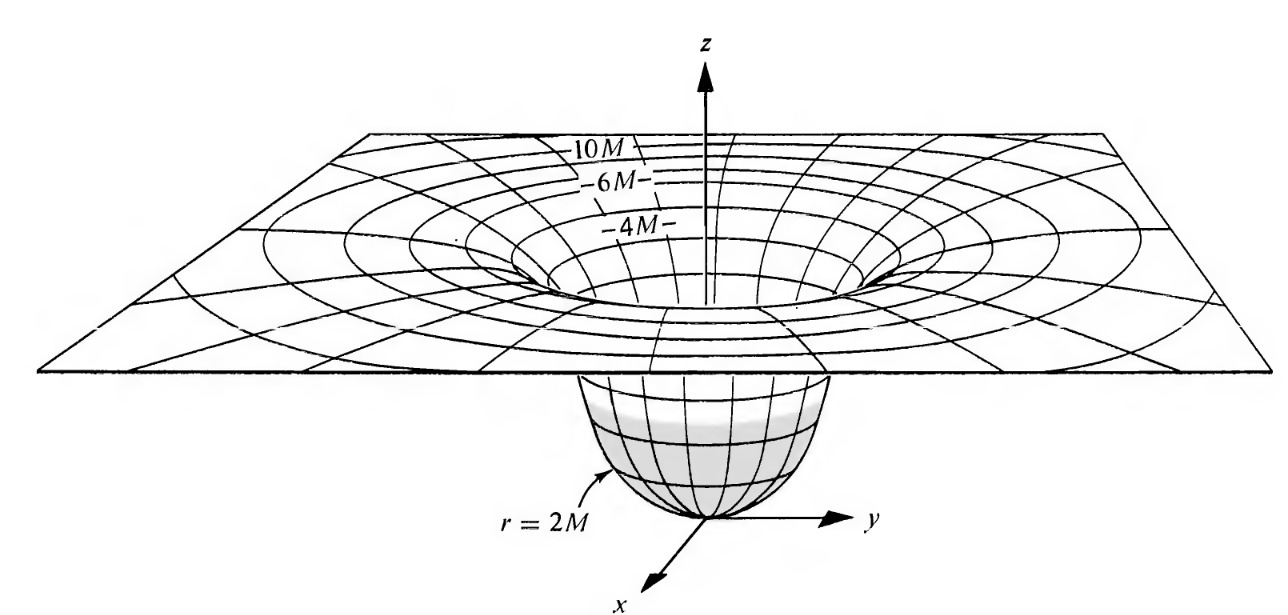
\includegraphics[width=0.7\linewidth]{Figuras/geometry-misner}
	\caption{Esquema de la geometría del espacio-tiempo de una estrella con simetría esférica. Tomado de \cite{misnerGravitation2017}.}
	\label{fig:geometry-misner}
\end{figure}

La solución general esférica (\ref{eq:metrica_esferica_general}) incluye varios casos de interés físico. En la región de vacío, cuando $T_{\mu\nu} = 0$, las ecuaciones de Einstein $G_{\mu\nu} = 0$ determinan completamente las funciones $\phi(r)$ y $\lambda(r)$, conduciendo a la solución exterior de Schwarzschild \cite{schwarzschildGravitationalFieldMass1999}. En el interior estelar, en presencia de materia con tensor de energía-momento (\ref{eq:tensor_fluido_perfecto}), las ecuaciones de Einstein proporcionan relaciones diferenciales entre $\phi(r)$, $\lambda(r)$, y las variables del fluido $\rho(r)$ y $P(r)$. En la superficie estelar, en $r = R$, las soluciones interior y exterior deben coincidir de manera continua, imponiendo condiciones de frontera específicas.

Para que la solución sea físicamente aceptable, las funciones métricas deben satisfacer condiciones de regularidad apropiadas. En el centro ($r = 0$) se requiere que $m(0) = 0$ y $\phi'(0) = 0$ para evitar posibles singularidades físicas o de coordenadas. En todo el espacio se debe cumplir que $e^{2\lambda} > 0$ y $e^{2\phi} > 0$ para mantener la signatura métrica consistentemente en el espacio-tiempo. En el infinito se exige que $\phi(\infty) = 0$ y $\lambda(\infty) = 0$ para recuperar la métrica de Minkowski, es decir, que en el infinito no haya influencia gravitacional de la estrella y el espacio-tiempo sea plano.

%Con la solución general esférica (\ref{eq:metrica_esferica_general}) y la parametrización de masa (\ref{eq:definicion_masa}) es posible derivar las ecuaciones de estructura que describen las propiedades al interior de las estrellas de neutrones y otros objetos compactos, como veremos en la siguiente sección.

\section{Ecuaciones de Estructura}

Las ecuaciones de estructura determinan la relación entre la distribución de materia en el interior de una estrella y la geometría del espacio-tiempo que genera. Para estrellas de neutrones, estas ecuaciones conectan las propiedades microscópicas de la materia densa con las características macroscópicas observables. En este sistema físico, el tensor de energía-momento del fluido perfecto (\ref{eq:tensor_fluido_perfecto}) actúa como fuente de las ecuaciones de Einstein (\ref{eq:einstein_field}). Las componentes del tensor de energía-momento en coordenadas esféricas son:

\begin{align}
	T_t^{\phantom{t}t} &= -\rho(r), \\
	T_r^{\phantom{r}r} &= T_\theta^{\phantom{\theta}\theta} = T_\varphi^{\phantom{\varphi}\varphi} = P(r).
\end{align}

Las ecuaciones de campo $G_{\mu\nu} = 8\pi T_{\mu\nu}$ establecen un sistema de ecuaciones diferenciales para las funciones métricas. Las componentes independientes son:

\begin{itemize}
	\item Componente $(t,t)$:
	\begin{equation}
		e^{-2\lambda}\left(\frac{2\lambda'}{r} - \frac{1}{r^2}\right) + \frac{1}{r^2} = 8\pi\rho.
		\label{eq:einstein_tt}
	\end{equation}
	\item Componente $(r,r)$:
	\begin{equation}
		e^{-2\lambda}\left(\frac{2\phi'}{r} + \frac{1}{r^2}\right) - \frac{1}{r^2} = 8\pi P.
		\label{eq:einstein_rr}
	\end{equation}
	\item Componente $(\theta,\theta)$:
	\begin{equation}
		e^{-2\lambda}\left[\phi'' + \phi'^2 - \phi'\lambda' + \frac{\phi' - \lambda'}{r}\right] = 8\pi P.
		\label{eq:einstein_theta}
	\end{equation}
\end{itemize}

Un resultado relevante para geometrías esféricamente simétricas es la posibilidad de expresar la función métrica $\lambda(r)$ en términos de una función de masa $m(r)$. Definiendo:

\begin{equation}
	e^{-2\lambda} = 1 - \frac{2m(r)}{r},
	\label{eq:definicion_masa}
\end{equation}

y utilizando esta parametrización en la ecuación (\ref{eq:einstein_tt}), obtenemos:

\begin{equation}
	\frac{dm}{dr} = 4\pi r^2 \rho(r),
	\label{eq:masa}
\end{equation}

donde la función $m(r)$ representa la masa inercial total contenida dentro de una esfera de radio $r$, y su interpretación física se hace clara al integrar la ecuación (\ref{eq:masa}):

\begin{equation*}
	m(r) = \int_0^r 4\pi r'^2 \rho(r') dr'.
\end{equation*}

Para sistemas asintóticamente planos como en este caso, la masa inercial coincide con la masa gravitacional activa del límite Newtoniano \cite{vollickMeaningVariousMass2021}, la cual contiene la masa en reposo total, la energía interna total y la energía potencial gravitacional dentro del radio $r$ \cite{misnerGravitation2017}. De la ecuación (\ref{eq:einstein_rr}) y usando la parametrización (\ref{eq:definicion_masa}), la función métrica $\phi(r)$ satisface:

\begin{equation}
	\frac{d\phi}{dr} = \frac{m + 4\pi r^3 P}{r(r - 2m)}.
	\label{eq:phi}
\end{equation}

La ecuación (\ref{eq:phi}) determina la componente temporal de la métrica una vez conocidas las funciones $m(r)$ y $P(r)$. Finalmente, utilizando (\ref{eq:definicion_masa}), (\ref{eq:masa}) y (\ref{eq:phi}) para sustituir $\phi''$, $\phi'$ y $\lambda'$ de (\ref{eq:einstein_theta}), obtenemos la ecuación de equilibrio hidrostático relativista, también llamada ecuación de Tolman-Oppenheimer-Volkoff (TOV) \cite{oppenheimerMassiveNeutronCores1939}:

\begin{equation}
	\frac{dP}{dr} = -\frac{(\rho + P)(m + 4\pi r^3 P)}{r(r - 2m)}.
	\label{eq:tov}
\end{equation}

Esta importante ecuación describe el equilibrio entre la presión del fluido y la atracción gravitacional, incluyendo correcciones relativistas necesarias para sostener objetos compactos y permitir su estabilidad. Para resolver el sistema de ecuaciones de estructura (\ref{eq:masa} - \ref{eq:tov}), se requiere de una ecuación de estado que relacione la presión y la densidad:

\begin{equation}
	P = P(\rho) \quad \text{o,} \quad \rho = \rho(P).
	\label{eq:ecuacion_estado}
\end{equation}

% Además, como condiciones de la estrella, se requiere tener una densidad central diferente de cero $\rho(0) = \rho_c > 0$ y se determina el limite exterior de la estrella $r = R$ como el punto donde la presión se anula $P(R) = 0$. En este punto, la masa total de la estrella es $M = m(R)$.

La solución se obtiene integrando numéricamente desde el centro hacia afuera, comenzando con una densidad central $\rho(0) = \rho_c > 0$ dada. El radio estelar $R$ se determina por la condición $P(R) = 0$, y la masa total $M = m(R)$ resulta de la integración de la ecuación de masa. En el límite no relativista ($M \ll R$ y $P \ll \rho$), la ecuación TOV se reduce a la ecuación clásica de equilibrio hidrostático:

\begin{equation}
	\frac{dP}{dr} = -\rho \frac{m}{r^2}.
\end{equation}

Para estrellas de neutrones, las correcciones relativistas en el sistema de ecuaciones son necesarias debido a su alta compacidad $M/R \sim 0.2-0.4$. Este sistema proporciona la base teórica para predecir las propiedades macroscópicas de las estrellas de neutrones a partir de modelos microscópicos de la materia nuclear densa.

\section{Observaciones de Estrellas de Neutrones}
\label{sec:obsNS}

Las observaciones astronómicas de estrellas de neutrones han experimentado una revolución en las últimas décadas \cite{pianMergersBinaryNeutron2021}, proporcionando restricciones cada vez más precisas sobre las propiedades de la materia densa. Estas mediciones permiten contrastar los modelos teóricos de ecuaciones de estado con la realidad física de estos objetos extremos. Las estrellas de neutrones se observan a través de múltiples canales electromagnéticos \cite{glendenningCompactStarsNuclear2000} y, recientemente, mediante ondas gravitacionales \cite{fonsecaNANOGravNineyearData2016}. Los principales métodos observacionales incluyen:

\begin{itemize}
	\item \textbf{Cronometraje de Pulsares}: Los pulsares son estrellas de neutrones altamente magnetizadas que emiten haces de radiación electromagnética. La precisión extrema en la medición de sus períodos de rotación permite determinar masas través del análisis orbital en sistemas binarios.
	
	\item \textbf{Astronomía de Rayos X}: Las estrellas de neutrones en sistemas binarios acretantes o como objetos aislados calientes pueden ser observadas en rayos X. Las misiones como NICER han revolucionado las mediciones de radio a través del modelado de puntos calientes superficiales.
	
	\item \textbf{Ondas Gravitacionales}: Las fusiones de estrellas de neutrones binarias, detectadas por LIGO-Virgo, proporcionan información sobre las propiedades de marea y la ecuación de estado a través de las modificaciones que introducen en la forma de onda gravitacional.
\end{itemize}

\subsection{Mediciones de Masa}

Las mediciones de masa de estrellas de neutrones se basan principalmente en el efecto Shapiro en sistemas binarios de pulsares. Este efecto relativista permite determinar las masas con alta precisión a partir del retraso temporal que experimenta la señal del pulsar al atravesar el campo gravitacional de su compañera.

Las mediciones más precisas incluyen:

\begin{itemize}
	\item \textbf{PSR J0740+6620}: Con una masa de $2.08 \pm 0.07 \, \masasol$ \cite{fonsecaRefinedMassGeometric2021}, representa la medición más precisa de una estrella de neutrones masiva.
	
	\item \textbf{PSR J0348+0432}: Una estrella de neutrones con masa $2.01 \pm 0.04 \, \masasol$ \cite{antoniadisMassivePulsarCompact2013}, crucial para establecer el límite inferior de la masa máxima.
	
	\item \textbf{PSR J0952-0607}: Con una masa reportada de $2.35 \pm 0.17 \, \masasol$ \cite{romaniPSRJ09520607Fastest2022}, aunque con mayor incertidumbre debido al método de determinación basado en espectrofotometría.
\end{itemize}

Estas observaciones establecen que las estrellas de neutrones pueden alcanzar masas superiores a $2 \masasol$, imponiendo restricciones sobre las ecuaciones de estado que deben ser suficientemente rígidas para soportar estas configuraciones. Otras estimaciones se han realizado empleando datos de ondas gravitacionales. Sin embargo, en mediciones mayores aún se discute la naturaleza del objeto observado (estrella de neutrones o agujero negro), como en el caso de GW190814 \cite{theligoscientificcollaborationGW190814GravitationalWaves2020, lopesNatureMassgapObject2022}, con una masa del objeto secundario estimado en $2.59^{+0.08}_{-0.09} \masasol$.

\subsection{Mediciones de Radio}

La misión NICER (Neutron star Interior Composition ExploreR) ha proporcionado algunas de las primeras mediciones simultáneas de masa y radio para estrellas de neutrones específicas. Estas mediciones se basan en el modelado de puntos calientes en la superficie de pulsares de milisegundo, analizando las modulaciones en el flujo de rayos X.

Los resultados más significativos incluyen, a 1$\sigma$ de confiabilidad:

\begin{itemize}
	\item \textbf{PSR J0740+6620}: Análisis independientes con NICER y X-ray Multi-Mirror han proporcionado valores $R = 13.7^{+2.6}_{-1.5}$ km \cite{millerRadiusPSRJ0740+66202021} y $R = 12.39^{+1.30}_{-0.98}$ km \cite{rileyNICERViewMassive2021};
	
	\item \textbf{PSR J0030+0451}: $M = 1.44^{+0.15}_{-0.14} \masasol$ y $R = 13.02^{+1.24}_{-1.06}$ km \cite{millerPSRJ0030+0451Mass2019};
	
	\item \textbf{PSR J0437-4715}: $M = 1.418 \pm 0.037 \masasol$ y $R = 11.36^{+0.95}_{-0.63}$ km \cite{choudhuryNICERViewNearest2024}.
\end{itemize}

Adicionalmente, se han realizado estimaciones de radio mediante la medición del parámetro de deformación de marea en ondas gravitacionales \cite{kumarTheoreticalExperimentalConstraints2024}. Sin embargo, para obtener estas estimaciones es necesario realizar modelamiento adicional, lo que hace esta estimación modelo-dependiente. Para el caso de \textit{GW190814} y asumiendo el objeto secundario como una estrella de neutrones de rotación rápida, se estimó un radio ecuatorial de $R_e = 14.1^{+1.5}_{-2.0}$ km, mientras que asumiendo una estrella no rotante, se estimó un radio canónico de $R_{1.4} = 13.3^{+0.5}_{-0.6}$ km, ambos en el intervalo de confianza a 90 \% \cite{biswasGW190814PropertiesSecondary2021}.\\


Las observaciones combinadas de masa y radio imponen restricciones consistentes sobre las posibles ecuaciones de estado de la materia nuclear densa. Estas restricciones pueden resumirse como:

\begin{itemize}
	\item \textbf{Rigidez Suficiente}: La ecuación de estado debe ser lo suficientemente rígida para soportar masas $\geq 2 \masasol$.
	
	\item \textbf{Radios Consistentes}: Los radios estelares deben estar en el rango $\sim 11-14$ km para masas típicas/canónicas de $\sim 1.4 \masasol$.
\end{itemize}

Estas restricciones observacionales permiten restringir las posibles ecuaciones de estado de la materia nuclear densa. Al resolver el sistema de ecuaciones de estructura (\ref{eq:masa} - \ref{eq:tov}) junto con una ecuación de estado específica (\ref{eq:ecuacion_estado}), es posible predecir la masa y radio de las estrellas de neutrones a partir de modelos microscópicos. De esta manera, las observaciones astronómicas establecen el puente entre la física microscópica de la materia nuclear densa y las características macroscópicas observables de estos objetos compactos, guiando la construcción y validación de modelos teóricos.

\begin{figure}[h]
	\centering
	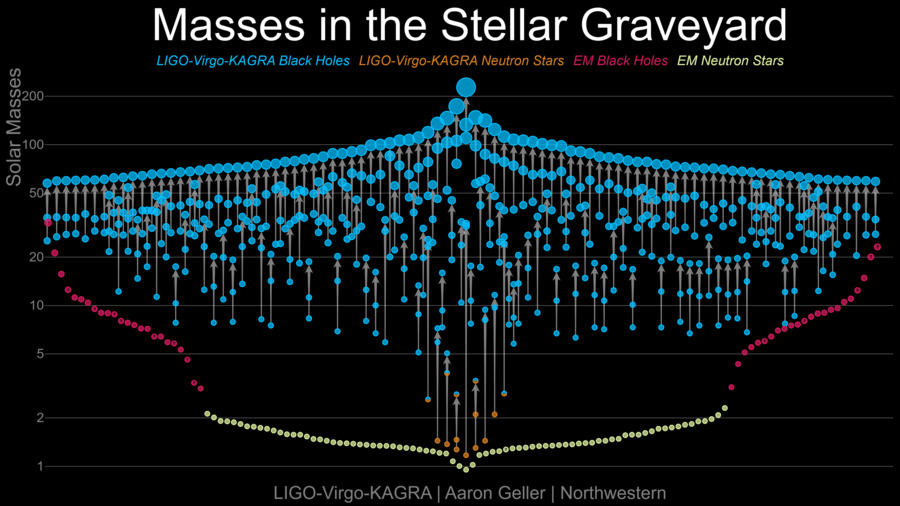
\includegraphics[width=0.7\linewidth]{Figuras/ligo-virgo-graveyard}
	\caption{Masas en el cementerio estelar. Contiene las masas estimadas mediante diferentes fuentes y su (posible) naturaleza, a enero de 2024. Tomado de \href{https://www.ligo.caltech.edu/image/ligo20250826d}{ligo.caltech.edu}.}
	\label{fig:ligo-virgo-graveyard}
\end{figure}

Las próximas generaciones de detectores de ondas gravitacionales, junto con misiones espaciales mejoradas y telescopios de nueva generación, prometen expandir significativamente nuestro conocimiento observacional de las estrellas de neutrones. Se espera que estas observaciones proporcionen restricciones aún más precisas sobre las ecuaciones de estado y posiblemente revelen nueva física en el régimen de densidades ultra-altas. Es claro que, a mayor número de observaciones, mayores son los requerimientos de nuestras teorías, lo que permite filtrar modelos físicos que pretendan describir la masa a densidades tan altas.
En particular, la detección de estrellas de neutrones con masas en el rango $2.5-3 \masasol$ o la confirmación de transiciones de fase en el interior estelar a través de observaciones de estrellas, prometen descubrimientos de impacto para nuestra comprensión de la materia nuclear densa. En la figura \ref{fig:ligo-virgo-graveyard} se pueden apreciar las estimaciones de masa hasta enero de 2024, así como la posible naturaleza del objeto. Cabe destacar que en el rango de 2 a 5$\masasol$ hay incertidumbre en la naturaleza de varios objetos detectados.


